\documentclass[]{cv-style} % Add 'print' in [] to get print-view
\usepackage{graphicx}
\begin{document}
\header{Beat }{Weber}
\begin{aside}
\section{.}
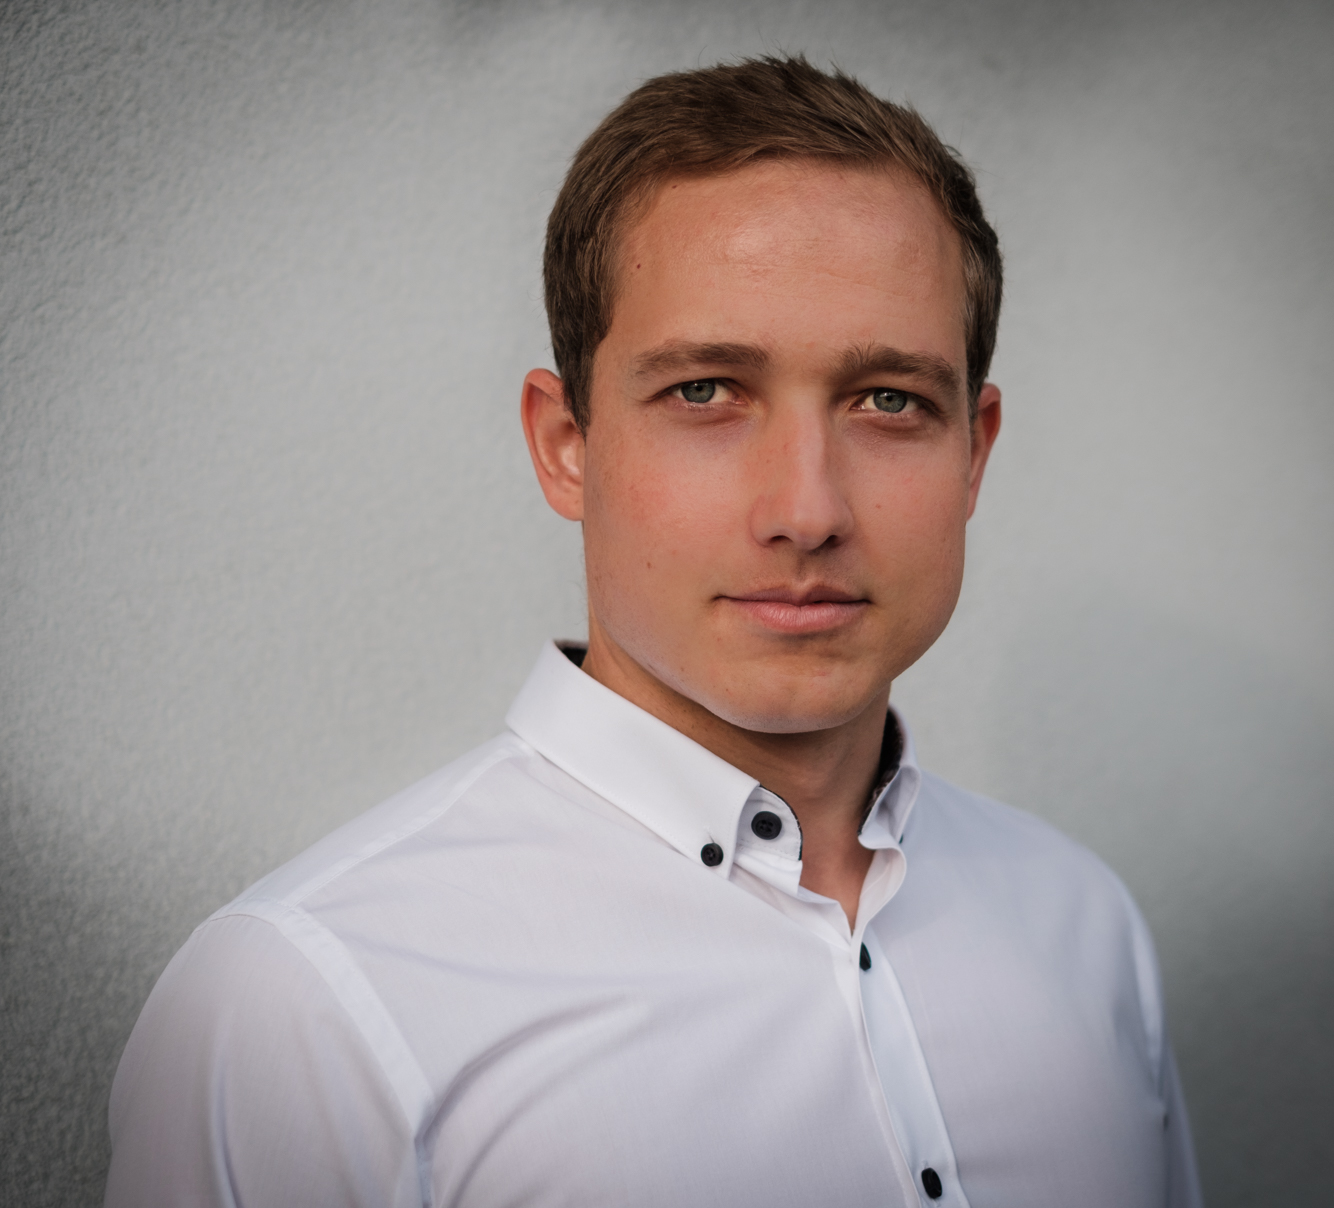
\includegraphics[width=4cm]{portrait}
\section{kontakt}
Winkelriedstrasse 47
6003 Luzern
~
16.05.1986
~
079 825 86 74
beat.weber.86@gmail.com
github.com/fonsie-lu
\section{sprachen}
Deutsch: Muttersprache
Englisch: Verhandlungssicher 
Französisch: Schulkenntnisse
\section{skills}
C\#, PowerShell, Java, JavaScript, SQL
\end{aside}
\section{motivation}
  \vspace{-0.3cm}
Ich möchte meine technischen Fähigkeiten als Software Engineer weiterentwickeln. Dabei bevorzuge ich Tätigkeiten im Bereich Front-end (JavaScript). Ich schätze eine offene und kritikfähige Teamkultur.
\section{berufserfahrung}
\begin{entrylist}
\entry
{2018 - 2019}
{Swisscom (Schweiz) AG}
{Luzern}
{\jobtitle{Software Engineer in Test}
\begin{itemize}
  \item Implementieren von Systemtest für Web mit JUnit, Selenium WebDriver und Ranorex (C\# und NUnit)
  \item Implementieren von System- und Integrationstests für Finnova Fat Client mit JUnit, OJDBC und Ranorex
\end{itemize}
.}
\entry
  {2011 - 2018}
  {Swisscom (Schweiz) AG}
  {Luzern}
  {\jobtitle{IT Consultant Application Manager}
\begin{itemize}
  \item Second Level Support für die Banking Software Finnova 
  \item Spezifizieren und Umsetzten von Service Request für Finnova
  \item Erheben von Auswertungen für Interne Zwecke (Monitoring und Reporting) und Externe Anfragen (SQL)
\end{itemize}
.}
\entry
  {2010}
  {Media Markt Kriens AG}
  {Kriens}
  {\jobtitle{Fachberater Neue Medien (Verkauf), 20\% Pensum}}\\
\entry
  {2005 - 2006}
  {Amt für Militär und Zivilschutz des Kantons Luzern}
  {Luzern}
  {\jobtitle{KV Praktikum}}\\
\entry
  {2004}
  {TEAMAG Immobilien AG Meggen}
  {Meggen}
  {\jobtitle{KV Praktikum}}
\end{entrylist}
\section{ausbildung}
\begin{entrylist}
\entry
{2007 - 2011}
{Hochschule Luzern - Wirtschaft}
{Luzern}
{Bachelor in Betriebsökonomie mit Vertiefung in Wirtschaftsinformatik}\\
\entry
{2007}
{Sprachaufenthalt}
{Whistler Canada}
{3-monatiger Sprachkurs}\\
\entry
{2006 - 2007}
{Militärdienst}
{Aarau}
{Durchdiener Füsilier}\\
\entry
{2003 - 2005}
{Wirtschafsmittelschule Luzern}
{Luzern}
{KV Ausbildung mit Berufsmatura}
\end{entrylist} 
\section{freizeit}
\begin{entrylist}
\entry
{}
{Sport}
{}
{Mountainbike, Rennrad, Klettern}\\
\entry
{}
{Kunst}
{}
{Interesse an Fotographie und Musikproduktion}
\end{entrylist}
\end{document}
